
\begin{figure*}
   \centering
      \ifscreen % macro TeX (issue de la classe report-rd-info.cls) permettant d'ajuster le contenu en fonction du l'orientation du document (<< screen >> ou pas)
         \rotatebox{90}{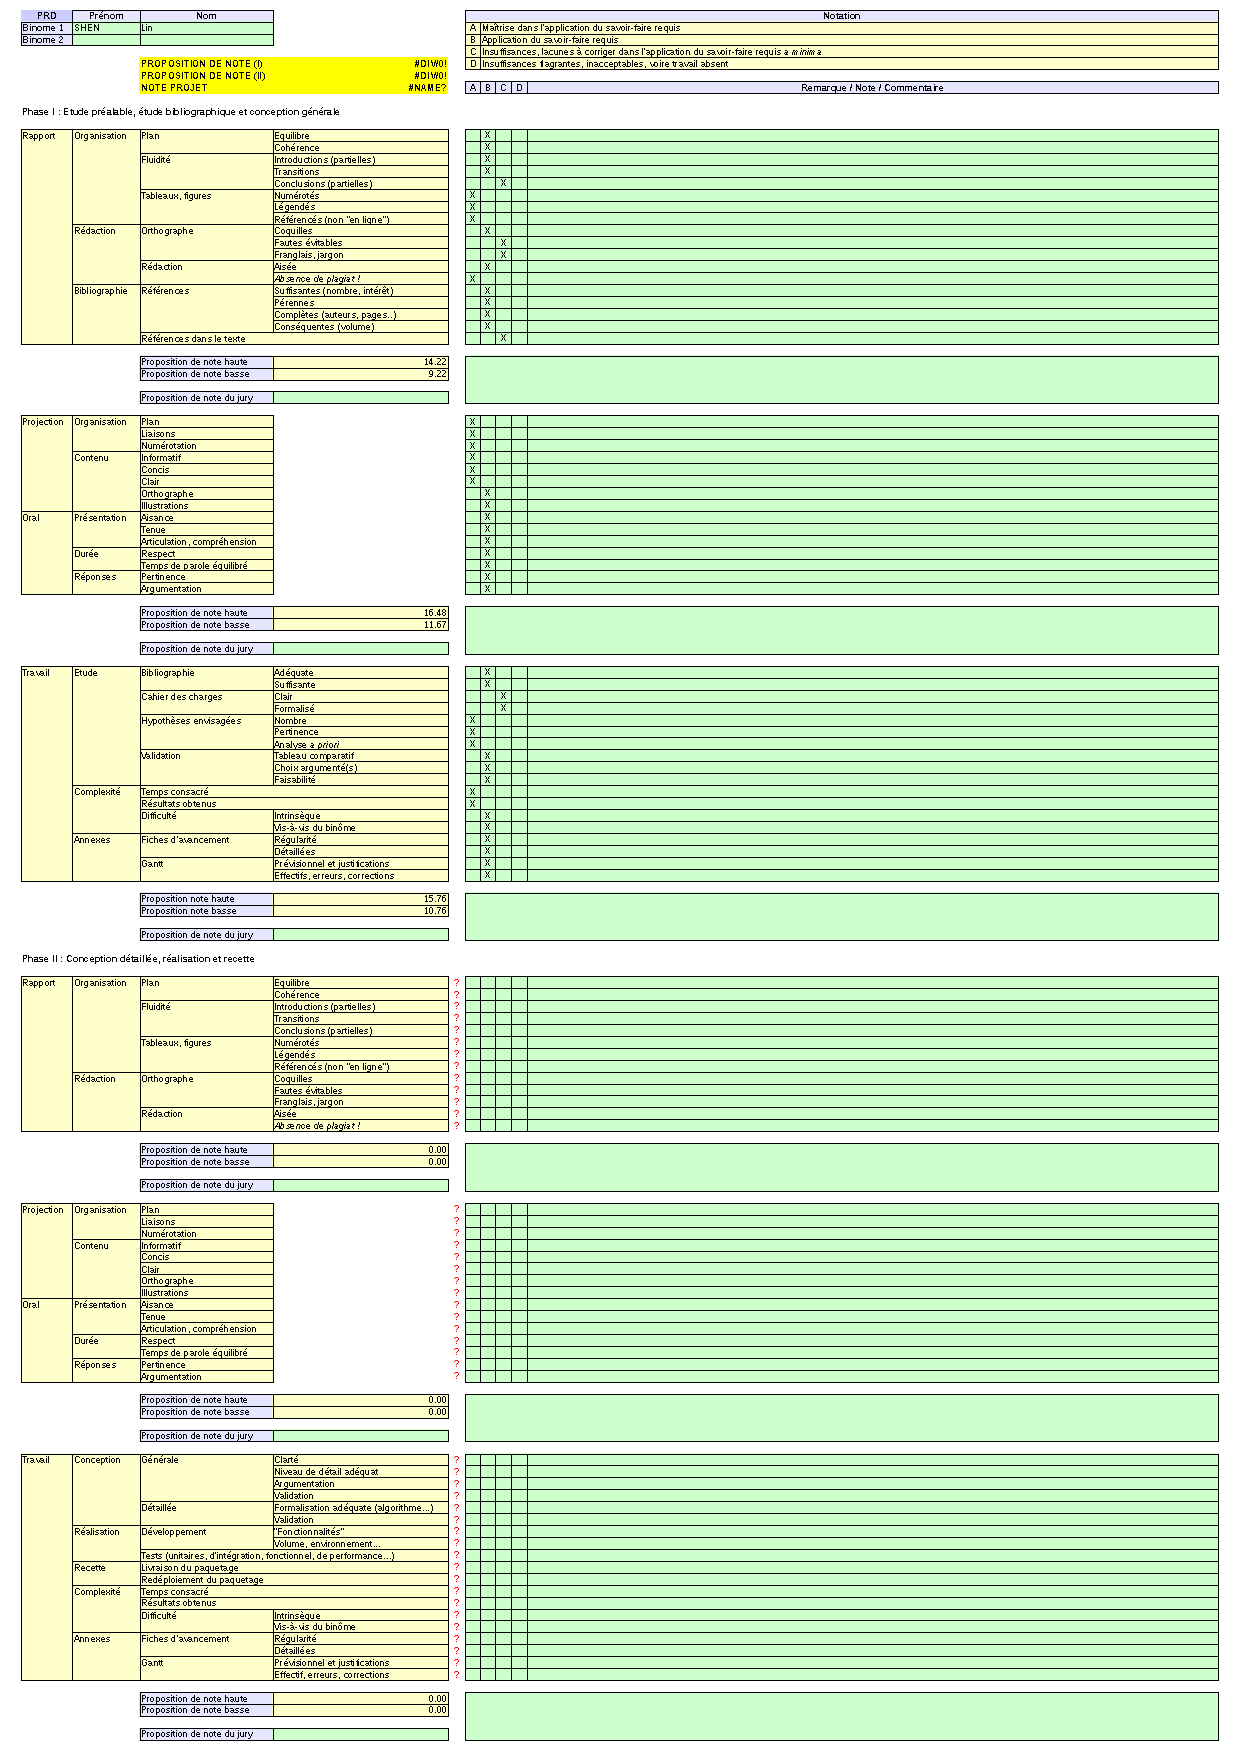
\includegraphics[width=0.9\textheight]{Images/auto-evaluation1}}
      \else
         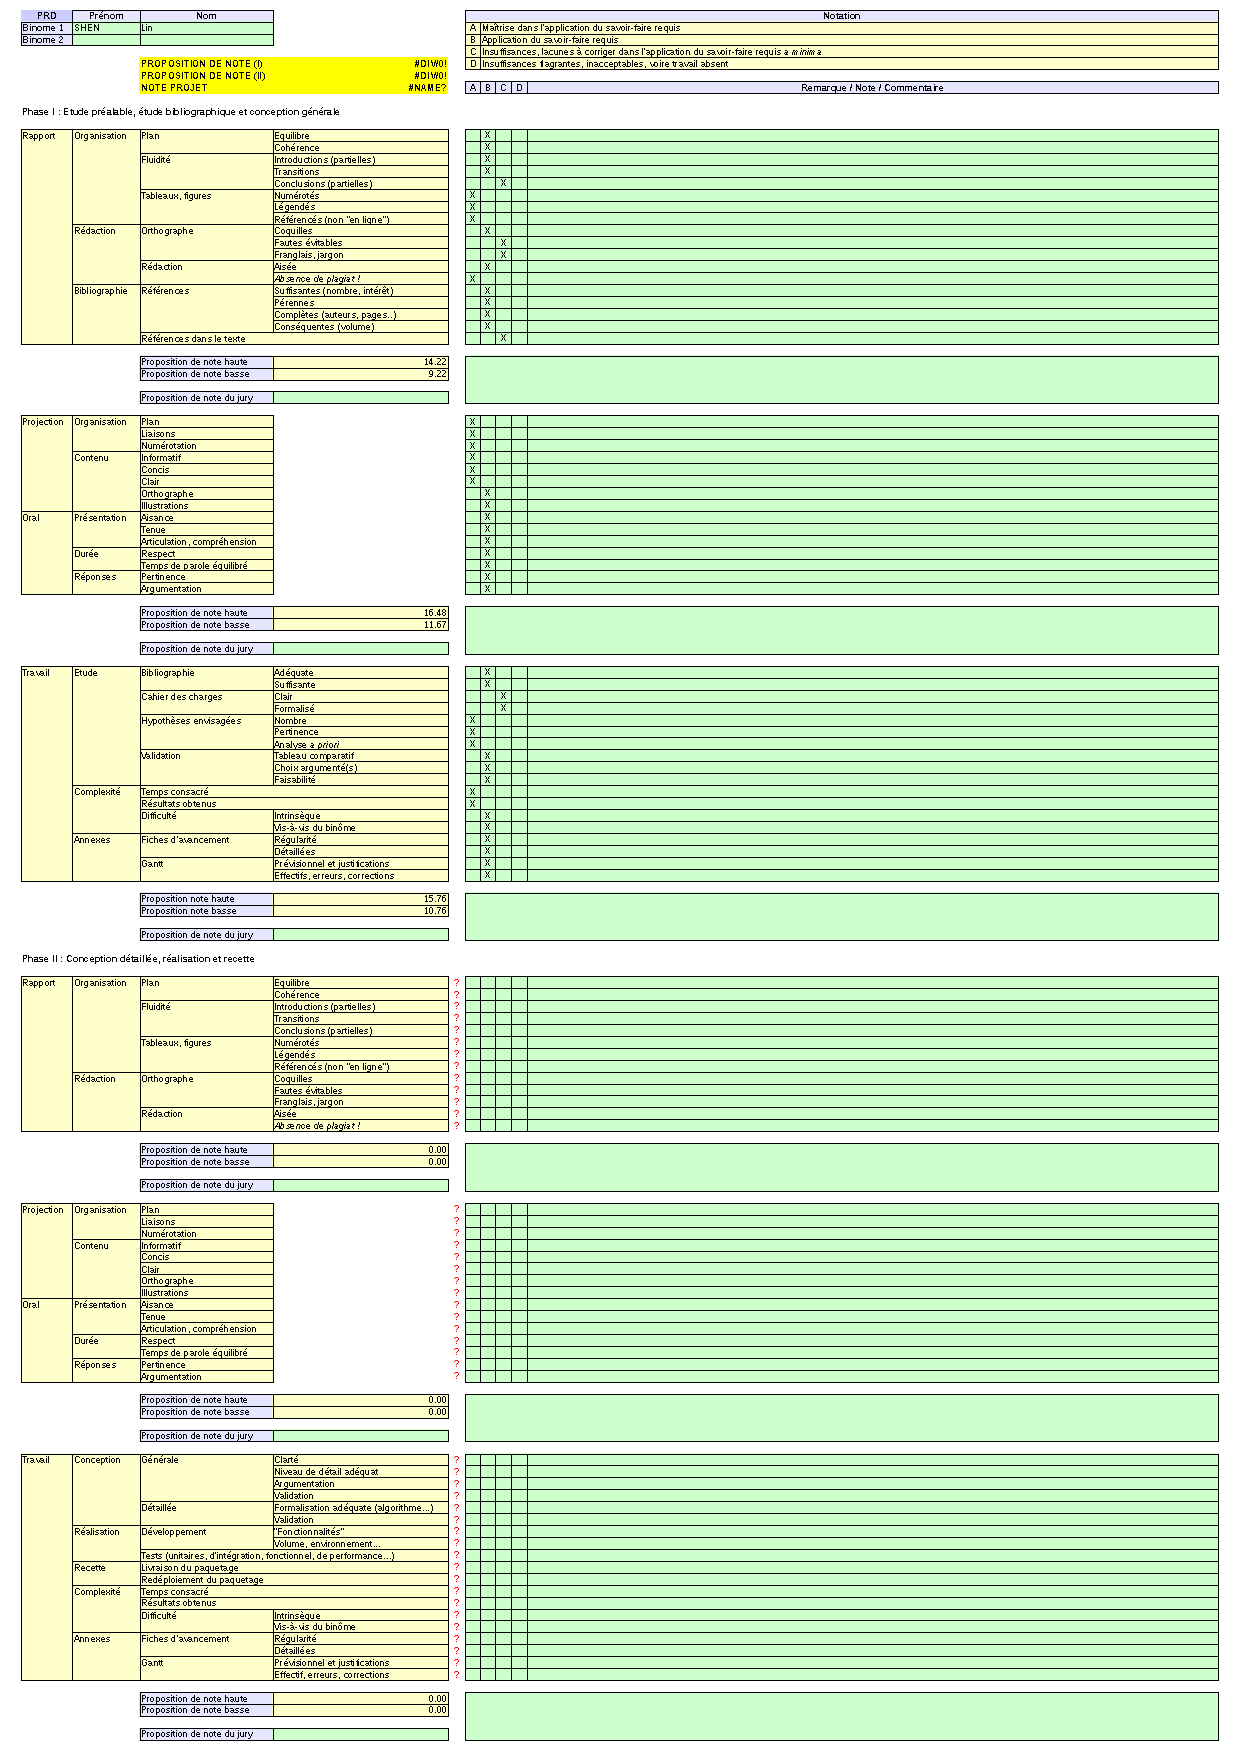
\includegraphics[width=0.9\textwidth]{Images/auto-evaluation1}
      \fi
   \caption{Auto evaluation}
   \label{fig:IntermediateAutoEvaluation}
\end{figure*}

\begin{comment}


Figure~\ref{fig:FinalAutoEvaluation} provides the same kind of evaluation for the second part of the project, i.e.:
\begin{enumerate}
   \item detailed design;
   \item development;
   \item receipt.
\end{enumerate}

\end{comment}
